% -----------------------------------------------
% Template for ISMIR Papers
% 2025 version, based on previous ISMIR templates

% Requirements :
% * 6+n page length maximum
% * 10MB maximum file size
% * Copyright note must appear in the bottom left corner of first page
% * Clearer statement about citing own work in anonymized submission
% (see conference website for additional details)
% -----------------------------------------------

\documentclass{article}
\usepackage[T1]{fontenc}
\usepackage[utf8]{inputenc}
\usepackage{ismir} % Remove the "submission" option for camera-ready version
\usepackage{amsmath,cite,url}
\usepackage{graphicx}
\usepackage{color}
\usepackage{booktabs}
\usepackage{placeins}
\usepackage{amssymb}% http://ctan.org/pkg/amssymb
\usepackage{pifont}% http://ctan.org/pkg/pifont

% \crefformat{footnote}{#2\footnotemark[#1]#3}

\usepackage{algorithm} % Added
\usepackage[noend]{algpseudocode} % Added
\usepackage{gensymb} % Added
\usepackage{siunitx} % Added
\usepackage{multirow} % Added
\usepackage{siunitx} % Added
\sisetup{input-symbols = ()} % Added
\usepackage{kotex}
\newcommand{\cmark}{\ding{51}}%
\newcommand{\xmark}{\ding{55}}%
\usepackage{microtype} % Added
\usepackage{paralist} % Added
\usepackage{float} % added

\newcommand{\alex}[1]{\textcolor{blue}{#1}}%
\newcommand{\jh}[1]{\textcolor{red}{#1}}

% Title. Please use IEEE-compliant title case when specifying the title here,
% as it has implications for the copyright notice
% ------
\title{Two Web Toolkits for Multimodal Piano Performance Dataset Acquisition and Fingering Annotation} %가제... 제목에 뭔가 GUI라는 약어를 써도 될지 좀 모르겠었어서 풀네임으로 적긴했었어요 ㅋㅋ 오 엄청 많네요 ㅎㅎ ㅋㅋ 그래서 일단은 줄여본,,!

%GUI 말고 pipeline 
% https://www.google.com/search?q=GUI+arxiv&rlz=1C5CHFA_enKR967KR970&oq=GUI+arxiv&gs_lcrp=EgZjaHJvbWUyBggAEEUYOTIICAEQABgWGB4yDQgCEAAYhgMYgAQYigUyDQgDEAAYhgMYgAQYigUyDQgEEAAYhgMYgAQYigUyBwgFEAAY7wUyBwgGEAAY7wUyCggHEAAYgAQYogQyCggIEAAYgAQYogTSAQgyNDUxajBqN6gCALACAA&sourceid=chrome&ie=UTF-8

% 한번 위 링크타고 검색! (케이스가 있는것 같더라구요 ㅋㅋ)

% Note: Please do NOT use \thanks or a \footnote in any of the author markup

% Single address
% To use with only one author or several with the same address
% ---------------
\multauthor
  {Junhyung Park$^\flat$ \hspace{1cm} Yonghyun Kim$^\natural$ \hspace{1cm} Joonhyung Bae$^\sharp$ \hspace{1cm} Kirak Kim$^\sharp$}
  {{\bfseries Taegyun Kwon$^\sharp$ \hspace{1cm} Alexander Lerch$^\natural$ \hspace{1cm} Juhan Nam$^\sharp$}\\
  $^\flat$ Department of Mathematical Sciences, KAIST, South Korea\\
  $^\natural$ Music Informatics Group, Georgia Institute of Technology, USA\\
  $^\sharp$ Graduate School of Culture Technology, KAIST, South Korea\\
  {\tt\small \{tonyishappy, jh.bae, kirak, ilcobo2, juhan.nam\}@kaist.ac.kr,}\\
  {\tt\small \{yonghyun.kim, alexander.lerch\}@gatech.edu}
  }
  
% For the author list in the Creative Common license, please enter author names.
% Please abbreviate the first names of authors and add 'and' between the second to last and last authors.

\def\authorname{J. Park, Y. Kim, J. Bae, T. Kwon, K. Kim, A. Lerch and J. Nam}

% Four or more addresses
% OR alternative format for large number of co-authors
% ------------
% \multauthor
%   {First author$^1$ \hspace{1cm} Second author$^1$ \hspace{1cm} Third author$^2$}
%   {{\bf Fourth author$^3$ \hspace{1cm} Fifth author$^2$ \hspace{1cm} Sixth author$^1$}\\
%   $^1$ Department of Computer Science, University, Country\\
%   $^2$ International Laboratories, City, Country\\
%   $^3$ Company, Address\\
%   {\tt\small CorrespondenceAuthor@ismir.edu, PossibleOtherAuthor@ismir.edu}
%   }

% For the author list in the Creative Common license, please enter author names.
% Please abbreviate the first names of authors and add 'and' between the second to last and last authors.

\sloppy % please retain sloppy command for improved formatting

\begin{document}

\maketitle % 여기서 에러가 왜 뜨는걸까요 흠... 그러게여.. (앞쪽에서 괄호가 덜닫혔나 살펴봤는데 그것도 아닌것 같구.. 신기쓰) author 쪽이 의심가긴 하는데 저도 잘 모르겠더라구요 ㅋㅋ (ㅋㅋ 일단은 보류..!! 렌더링하는데 문제는 없어보여서 ㅎㅎ)

\begin{abstract}
%The study of piano performance increasingly utilizes multimodal analysis to investigate the interplay between sound, physical movement, and artistic expression. However, progress in this domain is often constrained by the logistical challenges of creating large-scale datasets, such as data stream synchronization and the labor-intensive process of fingering annotation.
% To contribute to addressing these challenges, we present a toolkit comprising two graphical user interfaces: (i) PiaRec, which offers a system for the synchronized acquisition of audio, video, MIDI, and metadata, and (ii) ASDF, which provides an interface for the efficient, semi-automated annotation of performer fingering from video. By streamlining key stages of the data acquisition and annotation workflow, this toolkit aims to lower the barrier for producing large-scale multimodal datasets and foster further empirical research in music performance analysis.

%The computational study of piano performance using multimodal datasets offers deep insights into musical artistry and technique. However, the laborious process of acquiring large-scale multimodal data remains a significant bottleneck, hindering further progress in this field.

Piano performance is a multimodal activity, integrating acoustic output with the performer's complex physical actions and artistic interpretations. Despite growing research interest in analyzing the multimodal nature of piano performance, the laborious process of acquiring large-scale multimodal data remains a significant bottleneck, hindering further progress in this field. To overcome this barrier, we present an integrated web toolkit comprising two graphical user interfaces (GUIs): \begin{inparaenum}[(i)] \item PiaRec, which supports the synchronized acquisition of audio, video, MIDI, and performance metadata. \item ASDF, which enables the efficient annotation of performer fingering from the visual data. \end{inparaenum}Collectively, this system can streamline the acquisition of multimodal piano performance datasets.

%in the multimodal analysis of piano performance

% The inherently multimodal nature of piano performance, characterized by the complex interplay of sound, gesture, and artistic intent, has made it a compelling subject for empirical analysis. Yet, progress in this field is significantly hindered by the laborious process of acquiring large-scale, synchronized data. (제미나이)

%Piano performance is a multimodal activity, integrating acoustic output with the performer's complex physical actions and artistic interpretations. Despite growing research interest in this area, the laborious process of acquiring large-scale multimodal data remains a significant bottleneck, hindering further progress in this field.
  
% Despite growing research interest in this area, the complex and resource-intensive nature of data collection acts as a major impediment to new studies.

%process of acquiring datasets can hinder  ? data acquisition process for (research) can be laborious? acquiring large-scale multimodal datasets is a major bottleneck? laborious tedious cumbersome
% A significant bottleneck, however, constrains empirical inquiry into this relationship: the challenge of acquiring large-scale datasets that capture visual and fingering data. 
% impedes progress in this field

% Piano performance is a multimodal activity, integrating acoustic output with the performer's complex physical actions and artistic interpretations. Because of such nature, the interest for the multimodal piano performance dataset is growing for the relevant study in this domain. However, the laborious process of acquiring large-scale multimodal data remains a significant bottleneck, hindering further progress in this field.

% To overcome this barrier, we present an integrated web toolkit comprising two graphical user interfaces (GUIs): \begin{inparaenum}[(i)] \item PiaRec, which supports the synchronized acquisition of audio, video, MIDI, and performance metadata. \item ASDF, which enables the efficient annotation of performer fingering from the visual data. \end{inparaenum}Collectively, this system can streamline the acquisition of multimodal piano performance datasets.

% (원본)
% To broaden the application area of automatic music transcription, multimodal piano datasets today play an important role in the piano transcription task. Here we introduce two graphical user interfaces in Python environment, PiaRec and ASDF, which may assist in extending the visual and fingering modality of an audiovisual piano dataset. Given piano performance on digital piano with top-view video and audio record, they may help users to synchronize the data modalities and annotate fingering for a piano performance. Hence, they enable efficient large-scale multimodal data acquisition by utilizing both practice and performance sessions. The code and documentation of PiaRec and ASDF can be found from the author's Github page\footnote{https://github.com/yonghyunk1m/PianoVAM-Code}.
\end{abstract}

\section{Introduction}\label{sec:introduction}
%The computational study of piano performance as a multimodal activity offers deep insights into musical artistry and technique \cite{jensen2012multimodal, riley2005use, parmar2021piano}. However, progress in this field is often hindered by a substantial barrier: the logistical and technical challenges of acquiring large-scale datasets. These challenges include the synchronization of multimodal data streams and the meticulous logging of metadata.

%The computational study of piano performance as a multimodal activity offers deep insights into musical artistry and technique \cite{jensen2012multimodal, riley2005use, parmar2021piano}. Such research, particularly in fields like automatic music transcription and performance analysis, relies critically on synchronized multimodal datasets. However, existing acquisition methods require manual synchronization across multiple software tools and expert-level fingering annotation, creating significant barriers to large-scale dataset construction and broader research accessibility.

The computational study of piano performance as a multimodal activity offers deep insights into musical artistry and technique \cite{jensen2012multimodal, riley2005use, parmar2021piano}, making multimodal piano datasets combining audio, video, MIDI and fingering annotations play a crucial role. However, existing acquisition methods often require manual synchronization across multiple software tools and expert-level fingering annotation, limiting dataset scales and research accessibility.
% crucial for automatic transcription and performance analysis research. 

This difficulty is especially pronounced for fingering data. While fundamental to performance technique, the high degree of subjectivity in fingering makes it notoriously difficult to collect and analyze systematically \cite{swinkin2007keyboard}. To address these dataset acquisition and fingering annotation challenges, we introduce an integrated web toolkit, which consists of PiaRec and ASDF (a semi-Automated System for Detecting Fingering).\footnote{The source code will be released upon publication.} PiaRec automates the synchronized recording of multimodal data, while ASDF provides an efficient human-in-the-loop workflow to annotate fingering from the captured video.

This paper introduces an integrated system aimed at simplifying the dataset acquisition pipeline. By addressing the challenges of manual data synchronization and fingering annotation, we anticipate our work can contribute to the creation of large-scale multimodal piano datasets and support the empirical research that relies upon them.

%This paper introduces the integrated system to streamline the dataset acquisition pipeline from recording to annotation. We anticipate that Our work will expedite not only the creation of large-scale multimodal piano datasets but also the empirical research that relies upon them.
%We anticipate that by lowering these technical and logistical barriers, 

% (원본)
% In order to explore the intrinsic relationship between different modalities of piano performance, acquisition of multimodal piano dataset, especially audiovisual dataset is important. However, multiple procedures are required to collect audiovisual piano performance data, such as syncing audio and video files, recording metadata, and unifying various recording settings.\\
% To efficiently process all the preparation steps via graphical user interface, we propose PiaRec, a multimodal piano dataset recording system which (i) merges every step into few user inputs and (ii) unifies recording environments. %PiaRec also can be used to collect piano fingering data.\\ %PiaRec 관련 문단

% Many piano experts endeavored to discover the most efficient and expressive fingering for various piano techniques\cite{swinkin2007keyboard}. However, optimal piano fingering varies based on individual hand size, flexibility, musical interpretation, and desired dynamic nuances. This diversity of fingering makes the piano fingering generation task difficult.\\
% Here, we propose a GUI named ASDF, which stands for a semi-Automated System for Detecting Fingering, to capture the piano fingering information from the top-view piano performance video. ASDF can be applied to any performance midi data with top-view video, thus it can collect both various fingering attempts in practice sessions and also the elegant chain of fingerings of professional players. %We provide both user interfaces in the format of Streamlit package\cite{}.

\begin{figure}
    \centering
    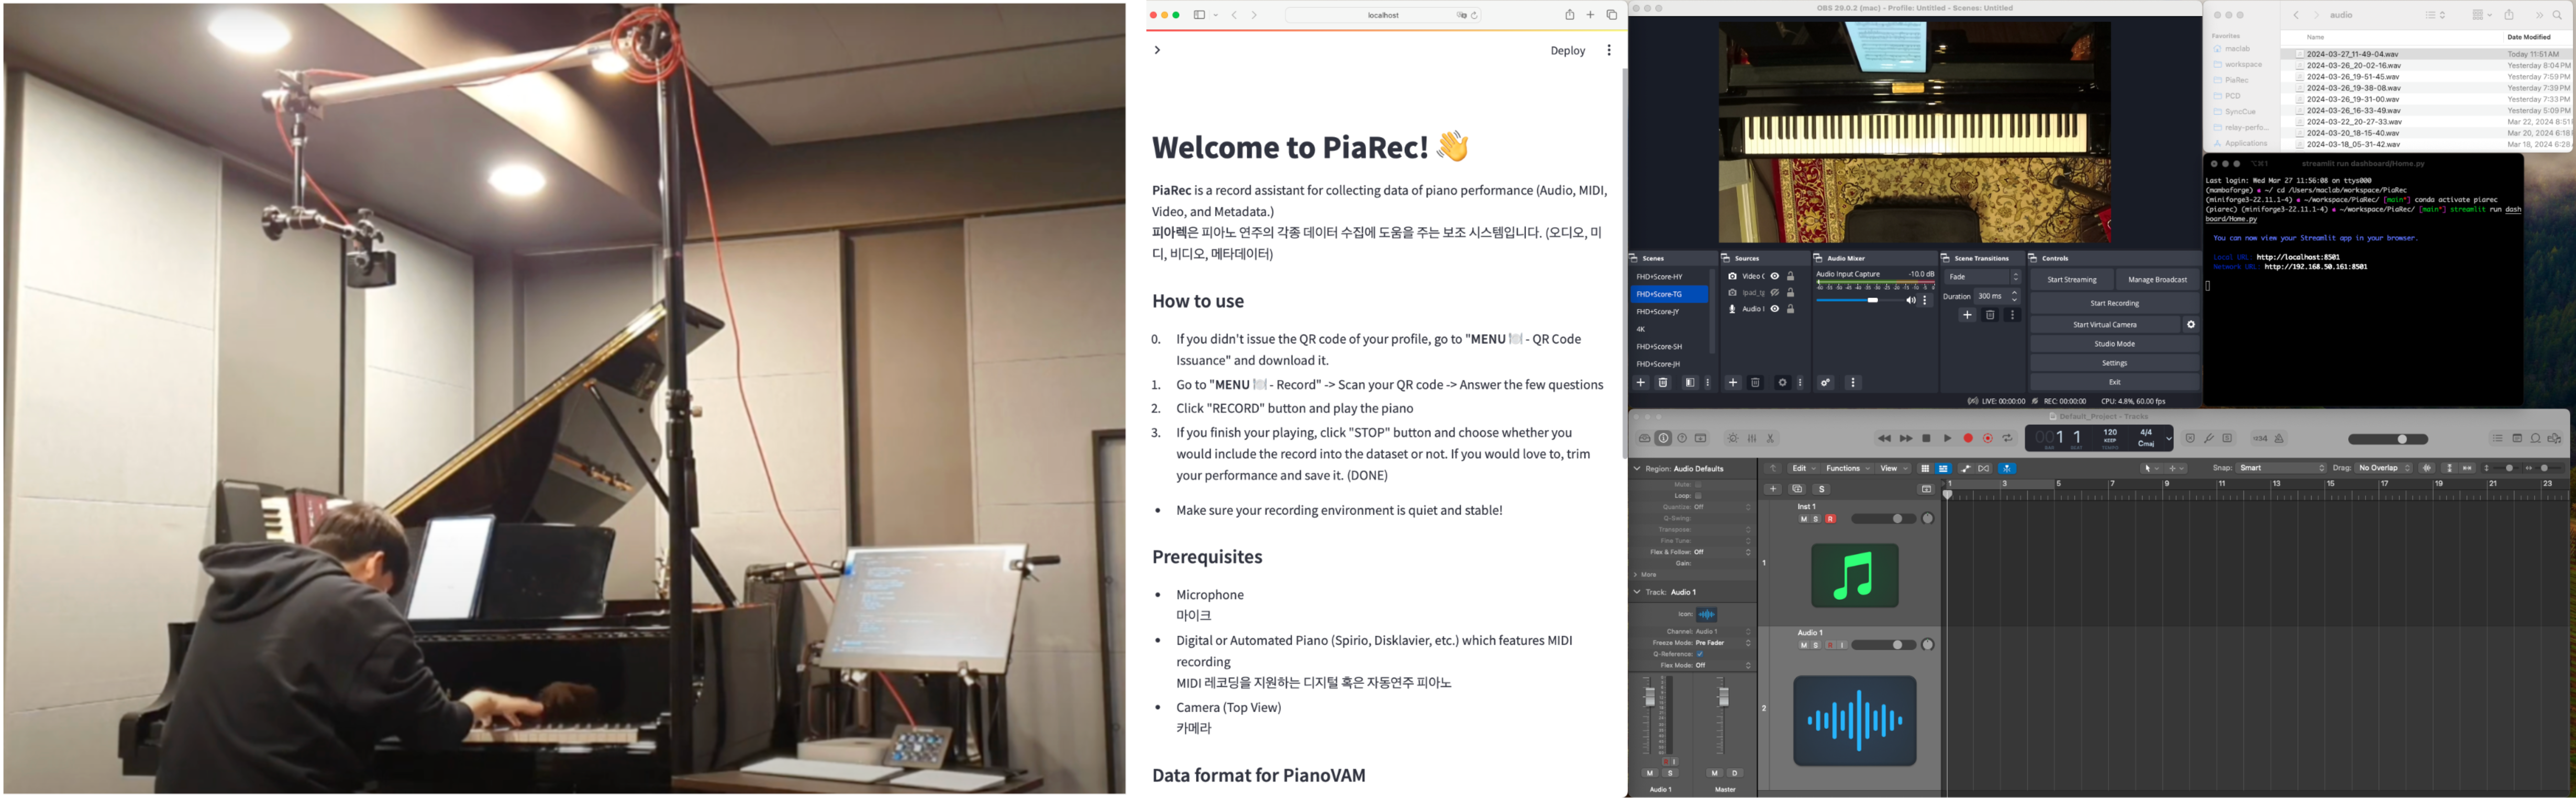
\includegraphics[width=\linewidth]{Images/PiaRec.png}
    \caption{PiaRec system in action, showing (left) the physical recording setup and (right) the PiaRec interface orchestrating OBS Studio and Logic Pro.}
    \vspace{-5mm}
    \label{fig:piarec}
\end{figure}

\section{PiaRec: GUI for Data Acquisition}
%PiaRec is a data collection system designed to easily gather synchronized audio, MIDI, video, and metadata from piano performances. It utilizes a Python-based graphical user interface (GUI) built with the Streamlit package to streamline the complex data acquisition process. The system requires standard hardware such as a digital piano with MIDI output, a microphone, and a top-view camera. For software control, PiaRec leverages the PyAutoGUI package to automate interactions with third-party recording applications. While the current implementation is optimized for Logic Pro and OBS Studio, its modular automation scripts are designed to be adaptable for other Digital Audio Workstations (DAWs) and video capturing systems with code modifications.

%PiaRec is a web-based system that automates synchronized recording of audio, MIDI, video, and metadata. Using QR codes for session control, it orchestrates Logic Pro, and OBS Studio through browser automation, eliminating manual synchronization errors while requiring only standard equipment (MIDI-equipped piano, camera, microphone).

PiaRec is a system designed to automate the synchronized acquisition of piano performance data, including audio, video, MIDI, and metadata. It features a graphical user interface (GUI) built with Python and Streamlit, which leverages the PyAutoGUI library to directly control external software like Logic Pro and OBS Studio, thereby eliminating manual synchronization errors. Notably, its modular design ensures extensibility, allowing it to be flexibly adapted for use with other Digital Audio Workstations and video capture systems.

% Users must install Logic Pro and OBS Studio in their system in order to use PiaRec. %마우스 클릭 매크로 같은것도 더 자동화 할 수 있으면 자동화 해야 할듯 합니다. (창 비율 설정에 따라 달라질 수 있기 때문)
\vspace{1.25mm}\text{}\\
\textbf{Workflow and Key Features.}\quad The PiaRec is centered around a web dashboard and a QR code-based control system. A first-time user completes a one-time registration on the ``Registration'' tab to generate three QR codes: (i) a \emph{Profile} code for user identification, (ii) a \emph{Play} code to initiate recording, and (iii) a \emph{Stop} code to terminate it.

For each recording session, the user inputs performance-specific metadata (e.g., composer, piece title) on the ``Record'' tab. Subsequently, scanning the \emph{Profile} and \emph{Play} codes triggers the automated, simultaneous recording of all data streams across Logic Pro and OBS Studio. The session concludes upon scanning the \emph{Stop} code, which terminates the session and saves the raw files.

Once the capture is complete, PiaRec performs its automated post-processing. It synchronizes the data streams by cross-correlating the audio from the different sources using the \texttt{numpy.correlate} function to find a precise time offset. This offset is used to trim the MIDI file, aligning it with the audio-visual data. Finally, all metadata is packaged with the synchronized files to create a well-structured data entry. %However, to ensure the highest precision, a final manual verification is recommended to identify potential MIDI jitter in the DAW for longer recordings.

% \subsection{Interface} 
% The interaction with the PiaRec system is centered around a web dashboard and a QR code-based control flow. A first-time user completes a one-time registration on the ``Registration'' page, entering data for a set of configurable metadata fields (e.g., age, gender, skill level). Upon submission, the system generates three QR codes for the user:
% \begin{inparaenum}[(i)]
%     \item A \emph{Profile} code containing the user's metadata.
%     \item A \emph{Play} code to initiate the recording sequence.
%     \item A \emph{Stop} code to terminate the recording sequence.
% \end{inparaenum}

% For each recording session, the user begins on the ``Record'' page to specify performance-related metadata, such as composer and piece title. Subsequently, the entire recording sequence is managed via a camera. The user first presents their \emph{Profile} code to be identified, followed by the \emph{Play} code to begin recording. The session concludes when the user presents the \emph{Stop} code.

% \subsection{Synchronization and Metadata Collection}
% PiaRec automates the capture and subsequent synchronization of the multimodal data streams. After the user fills in the performance metadata and scans the \emph{Profile} and \emph{Play} QR codes, PiaRec automatically starts MIDI and audio recording in Logic Pro while simultaneously starting video and audio recording in OBS. Once the performance is complete, scanning the \emph{Stop} QR code signals the system to cease and save all recordings.

% Following the capture process, the system aligns the data by cross-correlating the first 10 seconds of the clean audio from Logic Pro with the audio from the OBS video recording. Using the \texttt{numpy.correlate} function, it identifies the point of maximum similarity to determine the time offset between the two recordings. This calculated offset is then used to trim the MIDI file, ensuring it is aligned with the final audio-visual data. Finally, all collected metadata---from both the user's \emph{Profile} and the session's ``Record'' page---is packaged with the synchronized files, creating a well-structured data entry. However, given the potential for subtle MIDI drift during longer performances, a final manual verification of the alignment is recommended to ensure the highest data integrity and precision.

% The key feature of PiaRec is its automated synchronization function. It aligns the data by comparing the audio track recorded cleanly in Logic Pro with the audio track from the OBS video recording. The system calculates the time offset by applying the numpy.correlate function to the first 10 seconds of both audio sources. This cross-correlation identifies the point of maximum similarity, precisely determining the delay between the start of the two recordings. This offset is then used to trim the beginning and end of the MIDI file, ensuring it is perfectly synchronized with the final video and audio data. Finally, all collected metadata—both from the user's \emph{Profile} QR code and the Record page—is saved alongside the corresponding synchronized performance files.

% PiaRec collects metadata of the performance before it starts, including the piece information, so users must perform only a single piece.\\
%Sync details: 몇 ms 차이였는지 기억 안나는데 아마 한 프레임보단 작았던 것 같아요 10ms 정도였나?? 
%Face blur 이야기는 생각해 보니까 PianoVAM 얘기라 굳이 여기 넣을 필요는 없을 것 같아요

%Among the performers, one performer did not allowed the face reveal in the dataset. Hence \cite{pianovam} manually blurred the face region for the specfic performer, which is not contained in our UI.
\section{ASDF: GUI for Fingering Annotation}
% ASDF, which stands for ~~~ (Overview explanation)     <- 이걸 intro에 적긴 했는데 다시 한번 적는게 나을까요? (small 준형)
ASDF (semi-Automatic System for Detecting Fingering) is a toolkit for efficient piano fingering annotation, implemented with the Streamlit framework. It provides an interactive annotation interface for the hybrid workflow proposed by Kim et al. \cite{kim2025pianovam}, combining automated fingering detection algorithm with an intuitive interface for human verification.
\vspace{1.25mm}\\
\textbf{Workflow and Interface Design}\quad
%The ASDF interface guides the user through a three-stage workflow: %data preprocessing, automated candidate suggestion, and interactive manual annotation.
\vspace{1.25mm}\\
\textbf{1) Data Preprocessing:} A user begins by loading a performance video and its corresponding MIDI into the system. The first step The first step is spatial calibration of the keyboard area, performed via the ``Keyboard Detection'' tab. Here, the user defines the specific piano key locations within the video frame. This allows ASDF to map all 88 key regions and apply a heuristic correction for lens distortion by linear interpolation between keystones (see Figure \ref{fig:asdfkeyboard}). Next, the user initiates hand data extraction from the ``Generate Mediapipe Data'' tab. This backend process leverages the Mediapipe Hands \cite{arXiv20Zhang} and the floating hand detection algorithm from Kim et al. \cite{kim2025pianovam} to generate and save frame-wise skeleton data.\\
\textbf{2) Automated Candidate Suggestion:} Once preprocessing is complete, the user triggers the automated fingering analysis from the ``Pre-labeling'' tab. With a single action, the GUI executes the Fingering Candidate Selection Algorithm from Kim et al. \cite{kim2025pianovam}, which is described in Algorithm \ref{alg:fingeringalgo}. This algorithm processes the resulting MIDI and hand skeleton data to assign a likelihood score to each finger for every note, generating a set of probable fingering candidates.\\
\textbf{3) Interactive Annotation and Verification:} The core function of ASDF lies in its main ``Labeling'' tab, which is designed for efficient human-in-the-loop verification. This interface presents a synchronized, multi-panel view containing: \begin{inparaenum}[(i)] \item the performance video, \item a piano roll visualization of the MIDI notes, and \item a translucent overlay of the detected hand skeletons on the video. \end{inparaenum} Notes with a single, high-confidence candidate are pre-labeled, while notes with low confidence or multiple competing candidates are highlighted for manual review. A user can then click on any note in the piano roll to instantly navigate the video to that moment, visually verify the action, and assign or correct the fingering label with a simple input. This design significantly accelerates the annotation process by focusing human effort precisely where it is most needed.

% 원본
% \subsection{Interface}
% \textbf{Video preprocessing:} Users can extract framewise hand skeleton from the top-view video in the \textit{Generate Mediapipe Data} tab. ASDF also determines whether each detected hand skeleton is considered a \textit{floating hand}, which means the hand is in mid-air so that the hand cannot play any notes. Information of hand skeleton and floating state are saved in .pkl format. \\ % 헐 짱이다
% % Delete smart tempo 부분은 그냥 pre-finger labeling 코드 안에 집어넣고 삭제해도 될듯
% \textbf{Finger candidate calculation:} In the \textit{Pre-finger labeling} tab, ASDF decides the finger candidate for each note by Algorithm \ref{alg:fingeringalgo}.\\ %Tempo information of MIDI file is overwrited to 120 bpm.
% \textbf{Undecided fingering labeling:} Users can manually annotate the fingering number of undecided notes in the \textit{Label} tab.\\
% \textbf{Keyboard area detection \& normalization:} In order to match the location of the finger and corresponding key area for the fingering number annotation, specifying the location of the keyboard and the lens distortion of frame image must take place before the fingering annotation. In the \textit{Keyboard area detection} tab, users should manually designate the area of keyboard by clicking four vertex of the keyboard. The lens distortion of camera is calculated heuristically using quadratic approximation. \\ % 이 문단은 UI가 수정될 거라 그 이후에 다시 적어야 될 것 같아요

\begin{figure}
    \centering
    \includegraphics[width=\linewidth]{Images/ASDF_keyboard.png}
    \caption{ASDF interface for spatial calibration.}
    \label{fig:asdfkeyboard}  
    \vspace{-5mm}
\end{figure}

% \subsection{Algorithm \& Hyperparameters}
% Given top-view video and performance MIDI, ASDF decides the possible finger candidates for each note by Algorithm \ref{alg:fingeringalgo}, with floating hand information from the algorithm\cite{kim2025pianovam} based on hand skeleton detection via Mediapipe Hands\cite{arXiv20Zhang}. If there are no or multiple candidates, ASDF helps users to select the correct fingering on the label tab using visual assistance.
\begin{algorithm}[h!]
\caption{Fingering Candidate Selection Algorithm}\label{alg:fingeringalgo}
\begin{algorithmic}
\State $N = \text{Total number of notes}$
\State $K(n) = \text{Keyboard area of $n$th note}$
\State $I(n) = \text{Interval of video frames of $n$th note played}$
\State $H(f,i) = i\text{th finger location info of frame $f$,} $ but fingers of floating hands are not contained
\State $w = \text{width of a key}$ 
\State $S_n =$ Score of each finger likely playing $n$th note
\For{$n < N$}
\State $S_n \gets (0,\cdots,0)\in \mathbb{R}^{10}$
\For{$f \in I(n)$, $i<10$}
\If{\text{each }$H(f,i) \in K(n)$}
\State $S_n\gets S_n + \chi_i$ \Comment{$\chi_i$ = $i$th unit vector}
\ElsIf{$0<d(H(f,i),K(n))_{\mathbb{R}^2}< w$}
\State $S_n \gets S_n + \left(\frac{1-d(H(f,i),K(n))_{\mathbb{R}^2}}{w}\right)^{2}$
\EndIf
\EndFor
\EndFor
\For{$n<N$}
\If{$\exists i \ s.t. \ S_n \cdot \chi_i > 0.5|I(n)|$}
\If{$\exists ! \ i$}
\State Finger $i$ is the only candidate for $n$th note
\ElsIf{$\exists ! \ i \ s.t. \ S_n \cdot \chi_i > 0.8|I(n)|$}
\State Finger $i$ is the only candidate for $n$th note
\Else \text{ }  Multiple candidates for $n$th note
\EndIf
\Else \text{ } No candidate for $n$th note
\EndIf
\EndFor
\end{algorithmic}
\end{algorithm}
\vspace{-5mm}
\section{Conclusion}
We presented PiaRec and ASDF, the web toolkits designed to lower the significant barriers to creating richly annotated, multimodal piano performance datasets. This integrated pipeline streamlines the entire workflow---from synchronized data acquisition to efficient fingering annotation---providing a foundation for data collection that can be expanded in future work.
% 원본
% We present PiaRec and ASDF, which both aid the users who want to utilize the piano performance into an audiovisual dataset with the corresponding fingering annotations. The requirements for using PiaRec and ASDF are only a digital piano, a camera with a top-view position, and an audio recorder. This leads to a shorter preparation step for acquiring an audiovisual piano dataset, which enables MIR researchers to collect an audiovisual piano dataset for their study with less effort.

\section{Acknowledgments}
This research was supported by the National Research Foundation of Korea (NRF) funded by the Korea Government (MSIT) under Grant RS-2023-NR077289 and Grant RS-2024-00358448.

% For BibTeX users:
\bibliography{ISMIR2025_LBD}


\end{document}
